\chapter{Performance Enhancement}

One of the most commonly used approaches to mitigate covariate shift consequences is \textit{Reweighting}, which involves quantifying the degree of distribution shift and then apply a correction to the model \cite{zhang}. Another approach is \textit{Data Augmentation}, which consists of generating new data points from the original ones, in order to make the model more robust to the distribution shift \cite{zhao}. 

In this chapter we propose a robust training method which, in a preliminary analysis, seems to outperform the other models in terms of robustness to covariate shift.

This method is based on the idea of \textbf{Data Augmentation}. Instead of using training data as it is, we create new data applying the following transformation to the original data:

\begin{algorithm}[H]
    \caption{Custom Data Augmentation}
    \begin{algorithmic}[1]
        \Statex \textbf{Input:} $Data$, $N$
        \Statex \textbf{Output:} $Data_\text{aug}$
        \Statex
        \State $Size$ \leftarrow $len(Data)$ 
        \State $Data_\text{new}$ \leftarrow $Data$
        \State $Data_\text{tr}$ \leftarrow random subset of $N\%$ of $Data$
        \For{$x_i$ in $Data_\text{tr}$}
            \State $x_i' \leftarrow 
            \begin{cases}
                X_i + \varepsilon & \text{with probability } 0.5 \\
                X_i - \varepsilon & \text{with probability } 0.5
            \end{cases}$
            \State $y_i' \leftarrow y_i$
        \EndFor
        \State $Data_\text{aug} \leftarrow Data_\text{new} \cup Data_\text{tr}$
        \State $Data_\text{aug} \leftarrow Downsample(Data_\text{aug}, Size)$
        \State\Return $Data_\text{aug}$
    \end{algorithmic}
\end{algorithm}

Interestingly, this method does not require any knowledge of the shifted test distributions, it simply adds noise to a certain percentage of the training data. Then it downsamples the augmented data to the original size.
Despite the variation in the $x_i'$ values, the $y_i$ values remain the same, this leads to a \textbf{looser fit} on the training data and enhances the perfomance on the shifted test data.

\section{Experiments}
We firstly evaluated this method on the same classification task as the other models, but, since we needed a better way to theoretically understand the inner processes of the training, we decided to apply it to a simple 1-dimensional regression problem.

\subsection{Training Set}
The training set consists of 10,000 data points generated with $x$ values linearly spaced between -3 and 3, and $y$ values generated with the following formula:
\begin{equation}
    y = \sin(x)\exp(-x^2) + \varsigma
\end{equation}

Where $\varsigma$ is a random noise term drawn from a normal distribution with mean 0 and standard deviation 0.1.

\begin{figure}[H]
    \centering
    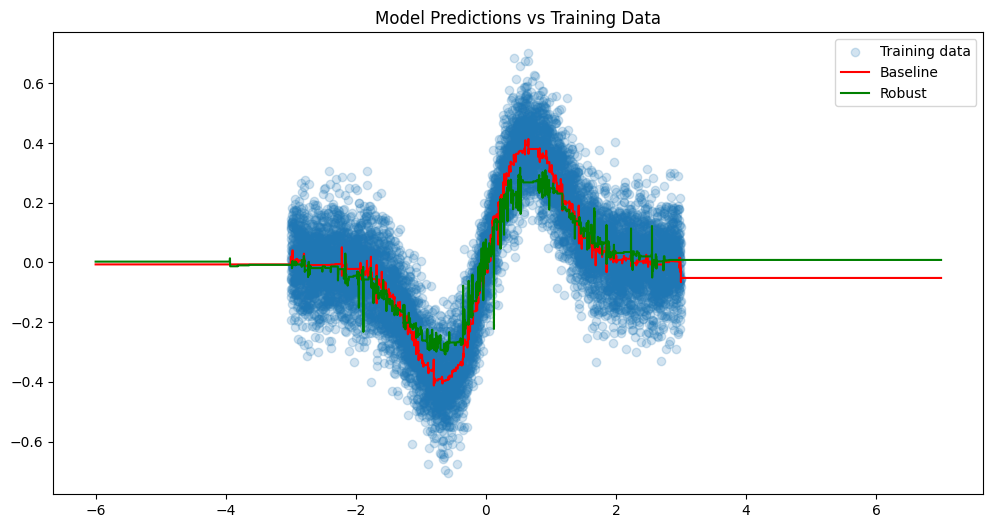
\includegraphics[width=0.8\textwidth]{assets/fit_on_train.png} 
    \caption{\textbf{Baseline and Robust models fit on the training data} To note that the robust model has a \textbf{looser fit} on the training data.}
    \label{fig:fit-train}
\end{figure}

\subsection{Test Sets}
Thirty test sets are created by shifting the $x$ values by factors ranging from 1.5 to 5.5. Each shifted test set is generated independently using the same underlying function and noise process as the training data.
\begin{figure}[H]
    \centering
    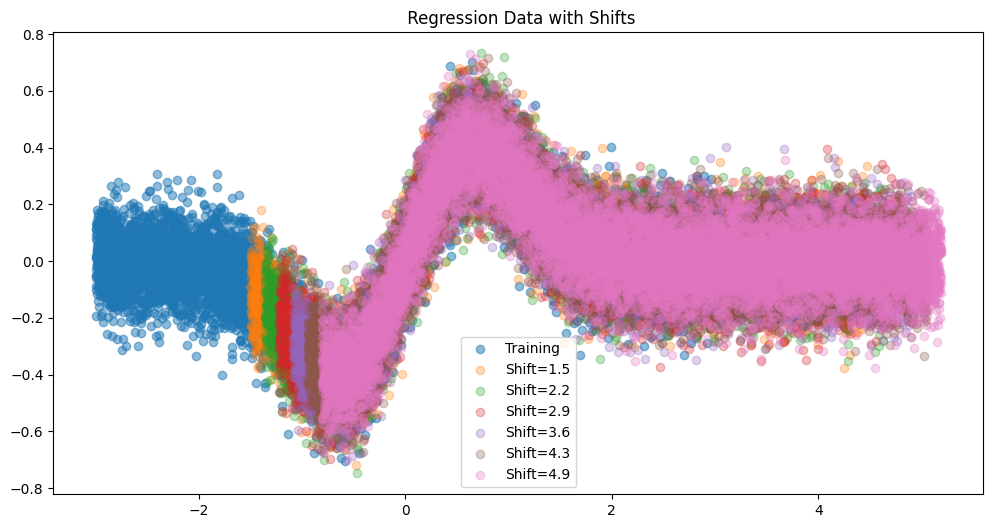
\includegraphics[width=0.8\textwidth]{assets/reg_shift_plot.png} 
    \caption{\textbf{A handful of test sets depicted together with the training set}}
    \label{fig:reg-shift-plot}
\end{figure}

\subsection{Models}
Two types of models are trained:
\begin{itemize}
    \item \textbf{Baseline Model}: A Gredient Boosting Regressor (GBR) is employed as a baseline model. The GBR is configured with the following hyperparameters: \plaintt{n\_estimators=100, max\_depth=5, learning\_rate=0.05}.
    \item \textbf{Robust Model}: The robust model has the same features as the baseline GBR but leverages the key parameters of the custom data augmentation method. The percentage of training data (\plaintt{fraction\_to\_shift}) to be augmented is set to 40\%. Meanwhile the \plaintt{base\_shift\_factor} controls the magnitude of shifts considered in training (set to 1 in this experiment).
\end{itemize}

\subsection{Results}

\subsubsection{Evaluation Metric}
The model performance is evaluated using the Mean Squared Error (MSE). For each shifted test set, the MSE is computed for both the baseline and robust models.
The improvement is defined as the relative reduction in MSE computed as :
\begin{equation}
    \text{Improvement} = \left(\frac{\text{MSE}_{\text{baseline}} - \text{MSE}_{\text{robust}}}{\text{MSE}_{\text{baseline}}}\right) \times 100\%
\end{equation}

The metric is computed for each shift, and the results are shown in the figure below.
\begin{figure}[H]
    \centering
    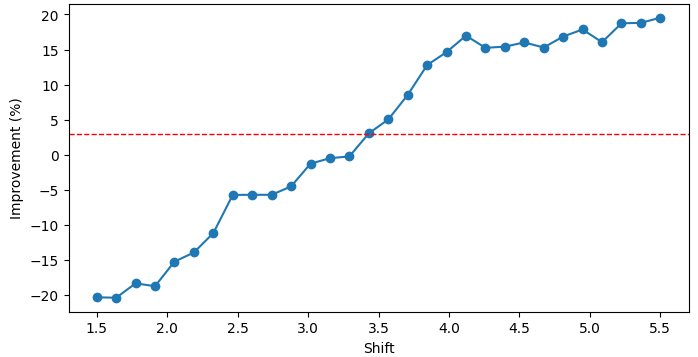
\includegraphics[width=0.8\textwidth]{assets/reg_exp_improvement.png} 
    \caption{\textbf{Model Improvement over Shifted Test Sets.} The red dotted line is the mean improvement across all shifts.}
    \label{fig:improv-plot}
\end{figure}

As we can see from the plot, the robust model has worse performance then the baseline model for relatively small shifts but as the shift in data points becomes more significant, the robust model outperforms the baseline model. The mean improvement across all shifts is still positive.
We believe the promising results of this methods are still to be analyzed in depth, but the preliminary results are encouraging.